\documentclass[a4paper,11pt]{article}
\usepackage[utf8]{inputenc}
\usepackage[english]{babel}
\usepackage[T1]{fontenc}
\usepackage{amsfonts}
\usepackage{amsmath}
\usepackage{amssymb}
\usepackage{tikz}
\usepackage{graphicx}
\usepackage{color}
\usepackage{pgfpages}
\usepackage[final]{pdfpages}
\usepackage[square,sort]{natbib}
\date{15 Octobre 2015} 
\title{Diagrame UML - fil rouge} 
\author{B. Pacreau, W. Peng, G. Soulié}

\begin{document}
\maketitle
\vskip 60pt
\section*{Notes à l'intention du lecteur :}
Vous trouverez en page 2 le diagramme UML avec uniquement les attributs des classes, donc sans les méthodes. pour ces deux diagrammes,
\begin{itemize}
\item Les méthodes get et set ne sont jamais représentés, pour gagner en lisiblité. Elles existent cependant pour pouvoir modifier certains attributs privés.
\item Les chemins complet de certains type ont étés ignorés. Ainsi, 
\begin{itemize}
\item List désigne java.util.List
\item Calendar désigne java.util.Calendar
\item String désigne java.lang.String
\item <item> désigne une liste d'items, sans pour autant que le type de la liste soit précisé.
\item Collection désigne java.util.Collection
\item ArrayList désigne java.util.ArrayList
\item etc...
\end{itemize}
\item Un temps de chargement parfois de quelque secondes est nécessaire pour charger les diagrammes.
\end{itemize}

\clearpage
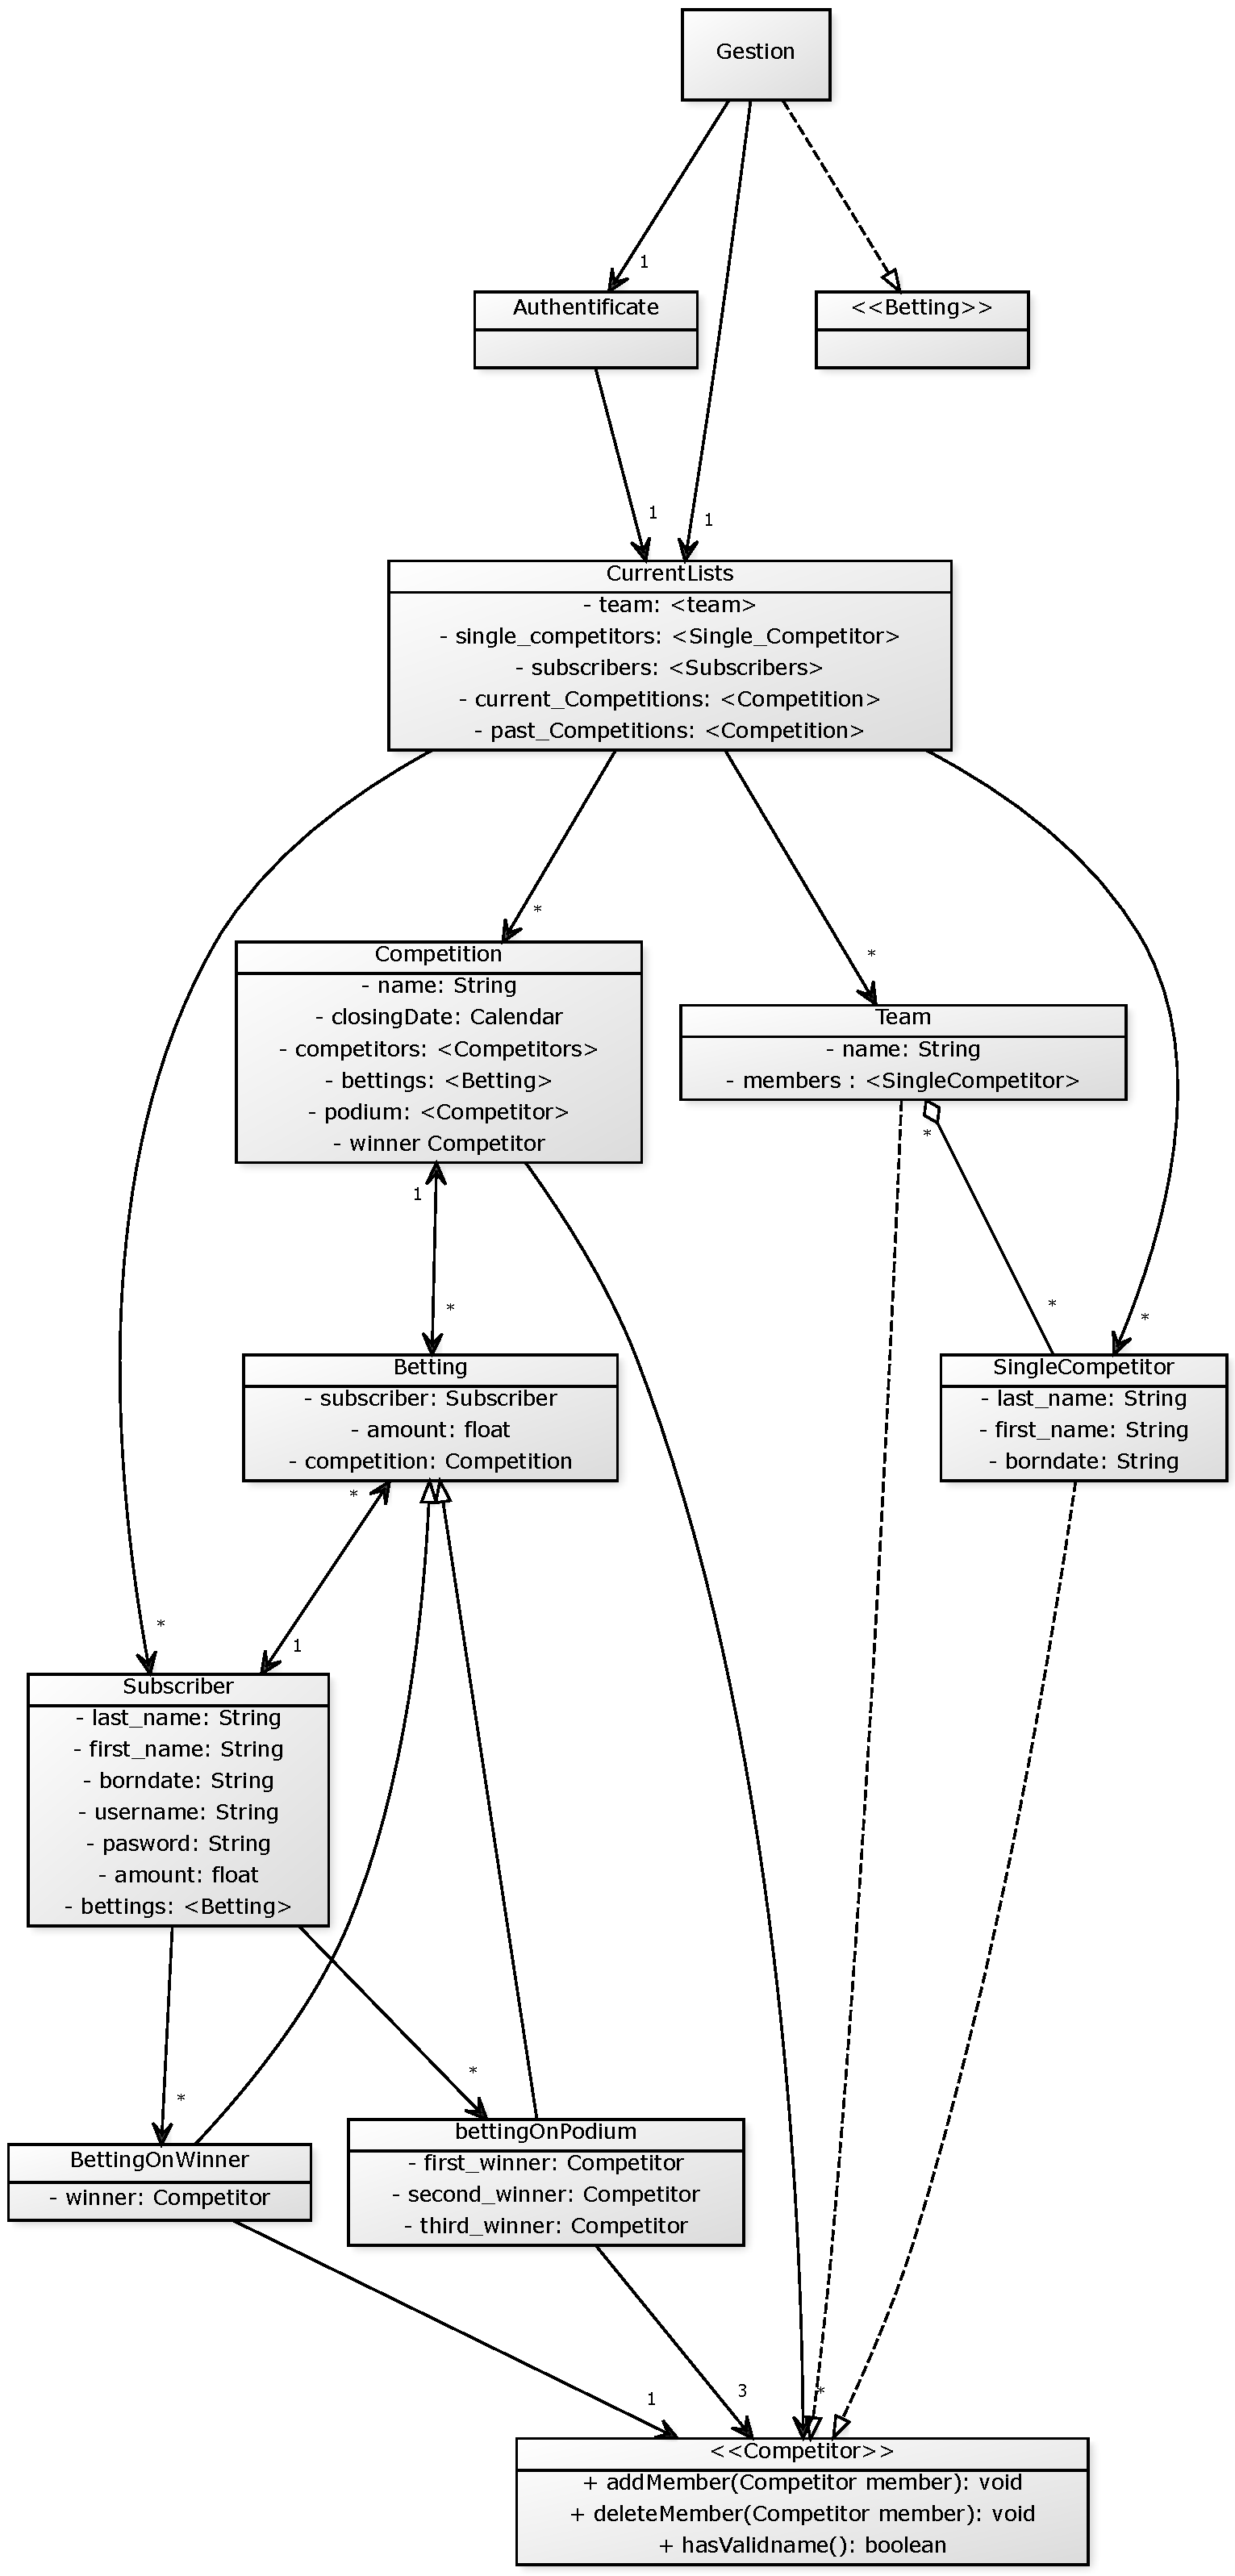
\includepdf[page=1]{p1.pdf}
\clearpage
\includepdf[page=1]{p2.pdf}


\end{document}